


\section{\highlight[id=Yuge]{Circle and Rectangle}}


For simplicity, the centroid of shape in Fig.~\ref{fig:simple_imgs} is
located at the center of the image, although periodic boundary
conditions can eliminate the boundary and translation effects. Circle
and rectangle are simple convex shapes without sophisticated geometric
features. Moreover, it is well-known that the rectangle perimeter is
longer than the circle circumference when their areas are
identical. Therefore, in theory, survival probabilities at short
times, i.e. number of steps $n$, of particles in the image with a
rectangle are smaller than a circle.


    \begin{figure}
      \centering
      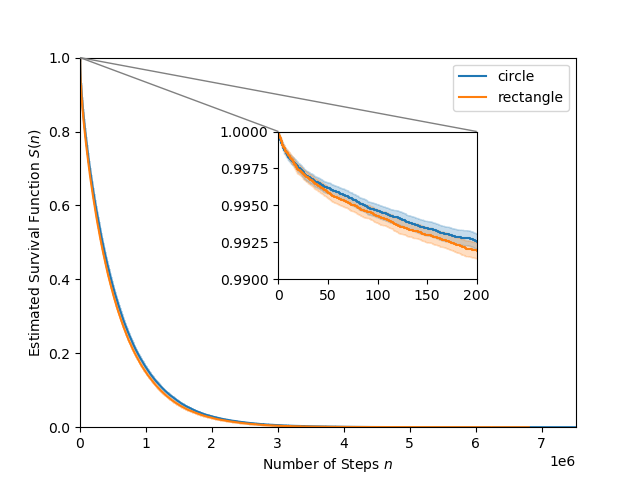
\includegraphics[width=\textwidth]{circle_rect_steps_sf.png}
      \caption{Since the survival curves for circle and rectangle overlap and cross, it is hard to detect the difference between them by eyes. However, the inset figure shows the greater details about the survival probabilities within the small number of steps. The area around the survival curve with the pale colour represents the $95\%$ confidence interval.}
      \label{fig:sf_simple_shape_steps}
    \end{figure}
     
Fig.~\ref{fig:sf_simple_shape_steps} shows the Kaplan-Meier estimates
and the $95\%$ confidence intervals for the survival functions,
$S(n)$, of circle and rectangle. Overall, the differences between
survival functions for the circle and rectangle are not
visible. Moreover, the approximated $95\%$ confidence intervals of the
survival functions overlap. However, an inset in
Fig.~\ref{fig:sf_simple_shape_steps} helps identify distinct
short-term behaviours of survival functions for circle and rectangle,
which are consistent with the theoretical results.





In this case, non-parametric statistical tests can be used to compare
entire survival distributions and assess their dissimilarities. The
logrank test has maximum power if the proportional hazards assumption
is satisfied.

   \begin{figure}
     \centering
     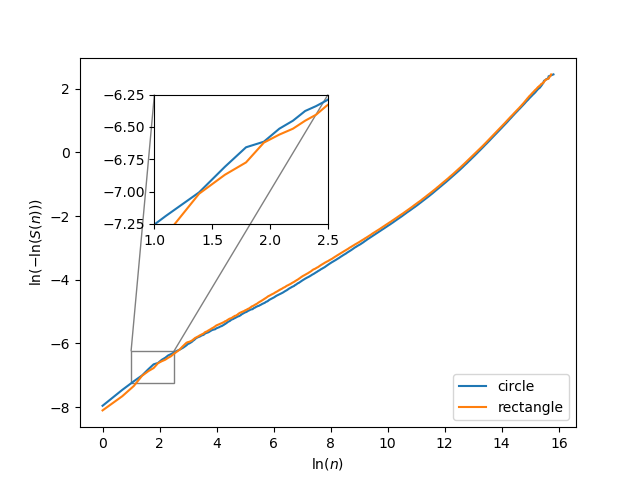
\includegraphics[width=\textwidth]{circle_rect_steps_ph.png}
     \label{fig:ph_test_simple_shapes}
     \caption{It is a graphical method for checking proportionality by looking for parallelism. As shown in the inset plot, two curves cross at some points and their shapes vary over time. Moreover, $p < 0.05$ in the non-proportional test. Thus, the survival functions for circle and rectangle do not satisfy the proportional hazard assumption.}
   \end{figure}


   \begin{table}
     \centering
     \begin{tabular}{lrr}
        \toprule
         {} &  test\_statistic &             p \\
         \midrule
         Logrank & 137.23 & 0.0 \\
         \midrule
         Tarone-Ware & 134.31 & 0.0 \\
         \midrule
         Gehan-Breslow & 123.83 & 0.0 \\
         \midrule
         Fleming-Harrington & 123.83 & 0.0 \\
         \bottomrule
     \end{tabular}
     \caption{Survival functions for circle and rectangle are statistically different since p values equal zeros.}
     \label{tab:test_simple_shape_steps}
   \end{table}



\subsection{Conclusion}


Although the proportional hazard assumption test is failed as shown in
Fig.~\ref{fig:ph_test_simple_shapes}, the weighted logrank tests
indicate that the null hypothesis should be rejected. In conclusion,
LRWs is an alternative tool to quantify and distinguish the geometries
in the $2-$ dimensional image without measuring the predefined shape
descriptors.
  
